\documentclass[11pt,a4paper]{article}

% ===== Kodowanie i jezyk =====
\usepackage[T1]{fontenc}
\usepackage[utf8]{inputenc}
\usepackage[polish]{babel}
\usepackage{lmodern}
\usepackage{microtype}

% ===== Uklad strony =====
\usepackage[a4paper,margin=2.3cm]{geometry}
\usepackage{fancyhdr}
\usepackage{lastpage}
\usepackage{setspace}
\setstretch{1.08}
\setlength{\headheight}{14pt}

% ===== Matematyka =====
\usepackage{amsmath,amssymb,amsfonts,amsthm,mathtools}
\usepackage{bm}

% ===== Grafika i kolory =====
\usepackage{graphicx}
\usepackage{float}
\usepackage[dvipsnames]{xcolor}
\usepackage{tikz}
\usetikzlibrary{arrows.meta,positioning,calc}
\usepackage[most]{tcolorbox}

% ===== Listy, tabele, linki =====
\usepackage{enumitem}
\usepackage{booktabs}
\usepackage{array}
\usepackage{hyperref}
\usepackage[nameinlink,noabbrev]{cleveref}

% ===== Algorytmy i kod =====
\usepackage{algorithm}
\usepackage{algpseudocode}
\usepackage{listings}

% ===== Kolory przewodnie =====
\definecolor{accent}{HTML}{0F4C5C}
\definecolor{accentsoft}{HTML}{E8F1F2}
\definecolor{accentline}{HTML}{8FB9C2}
\definecolor{warmgray}{HTML}{555555}
\definecolor{codebg}{HTML}{F7F7F5}

% ===== Linki =====
\hypersetup{
    colorlinks=true,
    linkcolor=accent,
    urlcolor=accent
}

% ===== Naglowki =====
\pagestyle{fancy}
\fancyhf{}
\lhead{\textsc{Uk\l ady dynamiczne}}
\chead{Kolokwium 1}
\rhead{19 kwietnia 2026}
\cfoot{\thepage/\pageref{LastPage}}
\renewcommand{\headrulewidth}{0.4pt}
\renewcommand{\footrulewidth}{0pt}

% ===== Ustawienia list =====
\setlist[itemize]{topsep=4pt,itemsep=2pt,leftmargin=1.8em}
\setlist[enumerate]{topsep=4pt,itemsep=2pt,leftmargin=2.1em}

% ===== Skróty matematyczne =====
\newcommand{\R}{\mathbb{R}}
\newcommand{\N}{\mathbb{N}}
\newcommand{\Z}{\mathbb{Z}}
\newcommand{\Q}{\mathbb{Q}}
\newcommand{\C}{\mathbb{C}}
\newcommand{\abs}[1]{\left\lvert #1 \right\rvert}
\newcommand{\norm}[1]{\left\lVert #1 \right\rVert}
\newcommand{\set}[1]{\left\{ #1 \right\}}
\newcommand{\seq}[1]{\left( #1 \right)}
\newcommand{\floor}[1]{\left\lfloor #1 \right\rfloor}
\newcommand{\Fix}{\operatorname{Fix}}
\newcommand{\Orb}{\operatorname{Orb}}
\newcommand{\Leb}{\lambda}
\newcommand{\modone}{\;(\operatorname{mod}\,1)}

% ===== Srodowiska twierdzen =====
\theoremstyle{plain}
\newtheorem{tw}{Twierdzenie}[section]
\newtheorem{lem}[tw]{Lemat}
\newtheorem{wn}[tw]{Wniosek}

\theoremstyle{definition}
\newtheorem{df}[tw]{Definicja}
\newtheorem{uw}[tw]{Uwaga}
\newtheorem{prz}[tw]{Przyk\l ad}

% ===== Tcolorbox =====
\tcbset{
    enhanced,
    breakable,
    boxrule=0.8pt,
    arc=2mm,
    colback=white,
    colframe=accent,
    left=1.2mm,
    right=1.2mm,
    top=1.0mm,
    bottom=1.0mm,
    before skip=10pt,
    after skip=10pt,
    pad at break*=1mm
}

\newtcolorbox{infobox}{
    colback=accentsoft,
    colframe=accentline,
    borderline west={1.2mm}{0pt}{accent},
    title=\textbf{Za\l o\.zenia robocze}
}

\newtcolorbox{opisbox}{
    colback=white,
    colframe=accentline,
    colbacktitle=accentsoft,
    coltitle=accent,
    title=\textbf{Opis zadania},
    fonttitle=\bfseries
}

\newtcolorbox{wynikbox}{
    colback=white,
    colframe=accent,
    title=\textbf{Wniosek},
    fonttitle=\bfseries
}

\newcounter{zadanie}
\newtcolorbox[auto counter,number within=section]{zadaniebox}[2][]{
    title={Zadanie~\thetcbcounter.\ifstrempty{#2}{}{ #2}},
    colback=white,
    colframe=accent,
    fonttitle=\bfseries,
    attach boxed title to top left={xshift=2mm,yshift*=-2mm},
    boxed title style={
        colback=accent,
        colframe=accent,
        sharp corners
    },
    #1
}

\newtcolorbox{rozwiazaniebox}{
    title=\textbf{Rozwi\k{a}zanie},
    colback=accentsoft!55!white,
    colframe=accentline
}

\newcommand{\stafflines}[2]{%
    \foreach \yy in {0,0.5,1,1.5,2} {
        \draw[gray!70] (0,{#1+\yy}) -- (#2,{#1+\yy});
    }
}

\newcommand{\quarternote}[2]{%
    \filldraw[fill=white] (#1,#2) ellipse (0.16 and 0.11);
    \draw ({#1+0.16},#2) -- ({#1+0.16},{#2+1.1});
}

\newcommand{\ledgernote}[2]{%
    \filldraw[fill=white] (#1,#2) ellipse (0.16 and 0.11);
    \draw ({#1-0.28},#2) -- ({#1+0.28},#2);
    \draw ({#1+0.16},#2) -- ({#1+0.16},{#2+1.1});
}

% ===== Listings =====
\lstdefinestyle{codestyle}{
    basicstyle=\ttfamily\small,
    backgroundcolor=\color{codebg},
    frame=single,
    rulecolor=\color{accentline},
    keywordstyle=\color{accent}\bfseries,
    commentstyle=\color{OliveGreen},
    stringstyle=\color{BrickRed},
    showstringspaces=false,
    breaklines=true,
    tabsize=4
}
\lstset{style=codestyle}

% ===== Tytuly sekcji =====
\usepackage{titlesec}
\titleformat{\section}
    {\Large\bfseries\color{accent}}
    {\thesection.}{0.6em}{}
\titleformat{\subsection}
    {\large\bfseries\color{accent}}
    {\thesubsection.}{0.5em}{}

% ===== Dokument =====
\title{\vspace{-1.5cm}\Huge\bfseries Kolokwium 1\\[0.4em]\Large Uk\l ady Dynamiczne}
\author{\large Pawe\l\ Drzyzga}
\date{19 kwietnia 2026}

\begin{document}

\raggedbottom

\pagenumbering{gobble}
\begin{titlepage}
    \centering
    \vspace*{2.5cm}
    {\Huge\bfseries\color{accent} Kolokwium 1\par}
    \vspace{0.4cm}
    {\LARGE Uk\l ady Dynamiczne\par}
    \vspace{1.2cm}
    {\large semestr letni 2025/2026\par}
    \vspace{2.2cm}
    \begin{tcolorbox}[width=0.82\textwidth,colback=accentsoft,colframe=accentline]
        \centering
        {\large\textbf{Opracowanie rozwi\k{a}za\'n zada\'n kolokwialnych}}\\[0.4em]
        \small
        Dokument zawiera kompletne rozwi\k{a}zania przygotowane w przejrzystej,
        zwartej i estetycznej formie matematycznej.
    \end{tcolorbox}
    \vfill
    {\large Autor opracowania: \textbf{Pawe\l\ Drzyzga}\par}
    \vspace{0.3cm}
    {\large Data: \textbf{19 kwietnia 2026}\par}
    \vspace{1.5cm}
\end{titlepage}

\clearpage
\pagenumbering{arabic}
\tableofcontents
\vspace{0.7cm}

\section{Zadanie 1}

\begin{opisbox}
Wybieramy kr\'otki utw\'or jednog\l osowy, przyjmujemy wysoko\'sci nut jako stany \l a\'ncucha Markowa,
liczymy przej\'scia mi\k{e}dzy kolejnymi d\'zwi\k{e}kami, wyznaczamy macierz przej\'scia, a nast\k{e}pnie
losujemy now\k{a} melodi\k{e} o tej samej d\l ugo\'sci.
\end{opisbox}

\begin{rozwiazaniebox}
\subsection*{1. Wyb\'or utworu i zapis nutowy}

Dla prostoty wybieramy uproszczony, jednog\l osowy wariant melodii \emph{Wlaz\l\ kotek na p\l otek}.
Rozpatrywany fragment zawiera \(24\) kolejne d\'zwi\k{e}ki, wi\k{e}c spe\l nia warunek zadania.

Dok\l adna sekwencja wysoko\'sci nut ma posta\'c
\[
\begin{aligned}
    (&G4,E4,E4,F4,D4,D4,C4,D4,E4,F4,G4,G4,\\
     &G4,G4,E4,E4,F4,D4,D4,C4,E4,G4,G4,C4).
\end{aligned}
\]

Poni\.zej zamieszczamy uproszczony zapis nutowy tej melodii.

\begin{center}
\begin{tikzpicture}[x=0.72cm,y=0.72cm]
    \stafflines{0}{13.8}
    \stafflines{-3.2}{13.8}
    \foreach \x in {4.2,8.4,12.6} {
        \draw[gray!70] (\x,-0.25) -- (\x,2.25);
        \draw[gray!70] (\x,-3.45) -- (\x,-0.95);
    }

    \quarternote{0.0}{1.0}
    \quarternote{1.2}{0.0}
    \quarternote{2.4}{0.0}
    \quarternote{3.6}{0.5}
    \quarternote{4.8}{-0.5}
    \quarternote{6.0}{-0.5}
    \ledgernote{7.2}{-1.0}
    \quarternote{8.4}{-0.5}
    \quarternote{9.6}{0.0}
    \quarternote{10.8}{0.5}
    \quarternote{12.0}{1.0}
    \quarternote{13.2}{1.0}

    \quarternote{0.0}{-2.2}
    \quarternote{1.2}{-2.2}
    \quarternote{2.4}{-3.2}
    \quarternote{3.6}{-3.2}
    \quarternote{4.8}{-2.7}
    \quarternote{6.0}{-3.7}
    \quarternote{7.2}{-3.7}
    \ledgernote{8.4}{-4.2}
    \quarternote{9.6}{-3.2}
    \quarternote{10.8}{-2.2}
    \quarternote{12.0}{-2.2}
    \ledgernote{13.2}{-4.2}
\end{tikzpicture}
\end{center}

\subsection*{2. Stany \l a\'ncucha Markowa}

Zgodnie z tre\'sci\k{a} zadania stanami \l a\'ncucha s\k{a} r\'o\.zne wysoko\'sci nut wyst\k{e}puj\k{a}ce
w melodii. W tym przyk\l adzie otrzymujemy zbi\'or stan\'ow
\[
    S=\set{C4,D4,E4,F4,G4}.
\]

W dalszej cz\k{e}\'sci zachowujemy powy\.zsz\k{a} kolejno\'s\'c stan\'ow w tabelach i macierzach.

\subsection*{3. Liczby przej\'s\'c pomi\k{e}dzy stanami}

Analizujemy kolejne pary s\k{a}siednich nut. Na przyk\l ad przej\'scie \(G4 \to E4\) wyst\k{e}puje
dwa razy, natomiast przej\'scie \(E4 \to F4\) wyst\k{e}puje trzy razy.

Macierz liczebno\'sci przej\'s\'c ma posta\'c
\[
N=
\begin{array}{c|ccccc}
     & C4 & D4 & E4 & F4 & G4 \\ \hline
    C4 & 0 & 1 & 1 & 0 & 0 \\
    D4 & 2 & 2 & 1 & 0 & 0 \\
    E4 & 0 & 0 & 2 & 3 & 1 \\
    F4 & 0 & 2 & 0 & 0 & 1 \\
    G4 & 1 & 0 & 2 & 0 & 4
\end{array}
\]

Suma element\'ow w kolejnych wierszach wynosi odpowiednio
\[
    2,\ 5,\ 6,\ 3,\ 7,
\]
co zgadza si\k{e} z liczb\k{a} wszystkich wyj\'s\'c z danego stanu.

\subsection*{4. Macierz przej\'scia otrzymanego \l a\'ncucha}

Prawdopodobie\'nstwa przej\'scia wyznaczamy przez normalizacj\k{e} wierszy macierzy \(N\), czyli
\[
    p_{ij}=\frac{n_{ij}}{\sum\limits_k n_{ik}}.
\]

Otrzymujemy macierz przej\'scia
\[
P=
\begin{array}{c|ccccc}
     & C4 & D4 & E4 & F4 & G4 \\ \hline
    C4 & 0 & \tfrac{1}{2} & \tfrac{1}{2} & 0 & 0 \\
    D4 & \tfrac{2}{5} & \tfrac{2}{5} & \tfrac{1}{5} & 0 & 0 \\
    E4 & 0 & 0 & \tfrac{1}{3} & \tfrac{1}{2} & \tfrac{1}{6} \\
    F4 & 0 & \tfrac{2}{3} & 0 & 0 & \tfrac{1}{3} \\
    G4 & \tfrac{1}{7} & 0 & \tfrac{2}{7} & 0 & \tfrac{4}{7}
\end{array}
\]

Ka\.zdy wiersz tej macierzy sumuje si\k{e} do \(1\), a wi\k{e}c rzeczywi\'scie jest to macierz
stochastyczna opisuj\k{a}ca rozpatrywany \l a\'ncuch Markowa.

\subsection*{5. Algorytm losowania kolejnych nut}

Now\k{a} melodi\k{e} generujemy wed\l ug nast\k{e}puj\k{a}cej procedury:
\begin{algorithm}[H]
\caption{Generowanie melodii z macierzy przej\'scia}
\begin{algorithmic}[1]
\State Ustaw nut\k{e} pocz\k{a}tkow\k{a} \(x_0\) jako pierwsz\k{a} nut\k{e} utworu oryginalnego
\State Dopisz \(x_0\) do nowej melodii
\For{$n=0,1,\dots,L-2$}
    \State Odczytaj wiersz macierzy \(P\) odpowiadaj\k{a}cy aktualnej nucie \(x_n\)
    \State Wylosuj kolejn\k{a} nut\k{e} \(x_{n+1}\) zgodnie z tym rozk\l adem prawdopodobie\'nstwa
    \State Dopisz \(x_{n+1}\) do nowej melodii
\EndFor
\end{algorithmic}
\end{algorithm}

W tym zadaniu przyjmujemy:
\begin{itemize}
    \item d\l ugo\'s\'c nowej melodii jest r\'owna d\l ugo\'sci melodii wyj\'sciowej, czyli \(L=24\),
    \item algorytm startuje od pierwszej nuty utworu oryginalnego, czyli od \(G4\),
    \item dla powtarzalno\'sci wyniku ustawiamy ziarno generatora losowego na \(20260420\).
\end{itemize}

\subsection*{6. Skrypt w Pythonie}

Aby zachowa\'c przejrzysto\'s\'c oraz pe\l n\k{a} odtwarzalno\'s\'c oblicze\'n, przygotowano skrypt
\texttt{scripts/zadanie1\_markov.py}. Program wykonuje nast\k{e}puj\k{a}ce kroki:
\begin{itemize}
    \item zapisuje melodi\k{e} wej\'sciow\k{a},
    \item wyznacza zbi\'or stan\'ow,
    \item liczy wszystkie przej\'scia mi\k{e}dzy kolejnymi nutami,
    \item normalizuje wiersze i buduje macierz przej\'scia,
    \item generuje now\k{a} melodi\k{e} o tej samej d\l ugo\'sci.
\end{itemize}

Najwa\.zniejsze fragmenty kodu nale\.zy rozumie\'c nast\k{e}puj\k{a}co:
\begin{itemize}
    \item \texttt{ORIGINAL\_MELODY} przechowuje analizowan\k{a} sekwencj\k{e} nut,
    \item funkcja \texttt{transition\_counts} zlicza przej\'scia \(n_{ij}\),
    \item funkcja \texttt{transition\_matrix} przekszta\l ca liczebno\'sci w prawdopodobie\'nstwa,
    \item funkcja \texttt{generate\_melody} losuje kolejne nuty zgodnie z odpowiednim wierszem macierzy \(P\).
\end{itemize}

Pe\l ny kod programu zamieszczono w aneksie na ko\'ncu dokumentu, aby by\l czytelny r\'ownie\.z w wersji PDF.

\subsection*{7. Wygenerowany nowy utw\'or}

Dla ustalonego ziarna generatora \texttt{20260420} skrypt zwraca nast\k{e}puj\k{a}c\k{a} melodi\k{e}:
\[
\begin{aligned}
    (&G4,E4,F4,G4,G4,C4,D4,C4,E4,F4,D4,C4,\\
     &E4,F4,G4,G4,G4,E4,E4,E4,G4,E4,F4,G4).
\end{aligned}
\]

Poni\.zej przedstawiamy jej uproszczony zapis nutowy.

\begin{center}
\begin{tikzpicture}[x=0.72cm,y=0.72cm]
    \stafflines{0}{13.8}
    \stafflines{-3.2}{13.8}
    \foreach \x in {4.2,8.4,12.6} {
        \draw[gray!70] (\x,-0.25) -- (\x,2.25);
        \draw[gray!70] (\x,-3.45) -- (\x,-0.95);
    }

    \quarternote{0.0}{1.0}
    \quarternote{1.2}{0.0}
    \quarternote{2.4}{0.5}
    \quarternote{3.6}{1.0}
    \quarternote{4.8}{1.0}
    \ledgernote{6.0}{-1.0}
    \quarternote{7.2}{-0.5}
    \ledgernote{8.4}{-1.0}
    \quarternote{9.6}{0.0}
    \quarternote{10.8}{0.5}
    \quarternote{12.0}{-0.5}
    \ledgernote{13.2}{-1.0}

    \quarternote{0.0}{-3.2}
    \quarternote{1.2}{-2.7}
    \quarternote{2.4}{-2.2}
    \quarternote{3.6}{-2.2}
    \quarternote{4.8}{-2.2}
    \quarternote{6.0}{-3.2}
    \quarternote{7.2}{-3.2}
    \quarternote{8.4}{-3.2}
    \quarternote{9.6}{-2.2}
    \quarternote{10.8}{-3.2}
    \quarternote{12.0}{-2.7}
    \quarternote{13.2}{-2.2}
\end{tikzpicture}
\end{center}

\end{rozwiazaniebox}

\begin{wynikbox}
Dla wybranego fragmentu melodii \emph{Wlaz\l\ kotek na p\l otek} otrzymali\'smy \l a\'ncuch Markowa
o zbiorze stan\'ow \(S=\set{C4,D4,E4,F4,G4}\) i macierzy przej\'scia \(P\) podanej powy\.zej.
Na podstawie tej macierzy, rozpoczynaj\k{a}c od nuty \(G4\), wygenerowali\'smy now\k{a} melodi\k{e}
o tej samej d\l ugo\'sci co utw\'or wyj\'sciowy. Kod programu zosta\l do\l \k{a}czony do opracowania,
wi\k{e}c ca\l e rozwi\k{a}zanie jest w pe\l ni odtwarzalne.
\end{wynikbox}

\section{Zadanie 2}

\begin{opisbox}
Rozwa\.zamy klasyczne przekszta\l cenie piekarza \(B \colon [0,1)^2 \to [0,1)^2\), wybieramy punkt
pocz\k{a}tkowy, wyznaczamy jego trajektori\k{e}, przedstawiamy kolejne obrazy rysunku oraz dowodzimy,
\.ze przekszta\l cenie zachowuje pole.
\end{opisbox}

\begin{rozwiazaniebox}
\subsection*{1. Wz\'or przekszta\l cenia piekarza}

Przyjmujemy standardow\k{a} posta\'c przekszta\l cenia piekarza:
\[
B(x,y)=
\begin{cases}
(2x,\tfrac{y}{2}), & \text{gdy } 0 \le x < \tfrac{1}{2},\\[0.3em]
(2x-1,\tfrac{y+1}{2}), & \text{gdy } \tfrac{1}{2} \le x < 1.
\end{cases}
\]

Geometrycznie oznacza to, \.ze kwadrat \([0,1)^2\) dzielimy na dwie pionowe po\l owy, ka\.zd\k{a}
rozci\k{a}gamy poziomo dwukrotnie, sp\l aszczamy pionowo dwukrotnie, a nast\k{e}pnie uk\l adamy jedn\k{a}
po\l ow\k{e} nad drug\k{a}.

\subsection*{2. Wyb\'or punktu pocz\k{a}tkowego}

Dla powtarzalno\'sci wyniku wybieramy punkt losowy przy u\.zyciu ziarna \texttt{20260420}. Otrzymujemy
\[
    (x_0,y_0)=(0.278662,\ 0.664184).
\]

\subsection*{3. Trajektoria punktu \((x_n,y_n)=B^n(x_0,y_0)\)}

Kolejne punkty trajektorii dla \(n=0,1,\dots,9\) wyznaczamy przez wielokrotne stosowanie odwzorowania
\(B\). Otrzymujemy:
\[
\begin{array}{c|cc}
n & x_n & y_n \\ \hline
0 & 0.278662 & 0.664184 \\
1 & 0.557325 & 0.332092 \\
2 & 0.114649 & 0.666046 \\
3 & 0.229299 & 0.333023 \\
4 & 0.458597 & 0.166511 \\
5 & 0.917194 & 0.083256 \\
6 & 0.834389 & 0.541628 \\
7 & 0.668777 & 0.770814 \\
8 & 0.337555 & 0.885407 \\
9 & 0.675109 & 0.442703
\end{array}
\]

Na rysunku poni\.zej zaznaczono wszystkie te punkty w kwadracie \([0,1]^2\) i po\l \k{a}czono kolejne
wyrazy trajektorii odcinkami.

\begin{center}
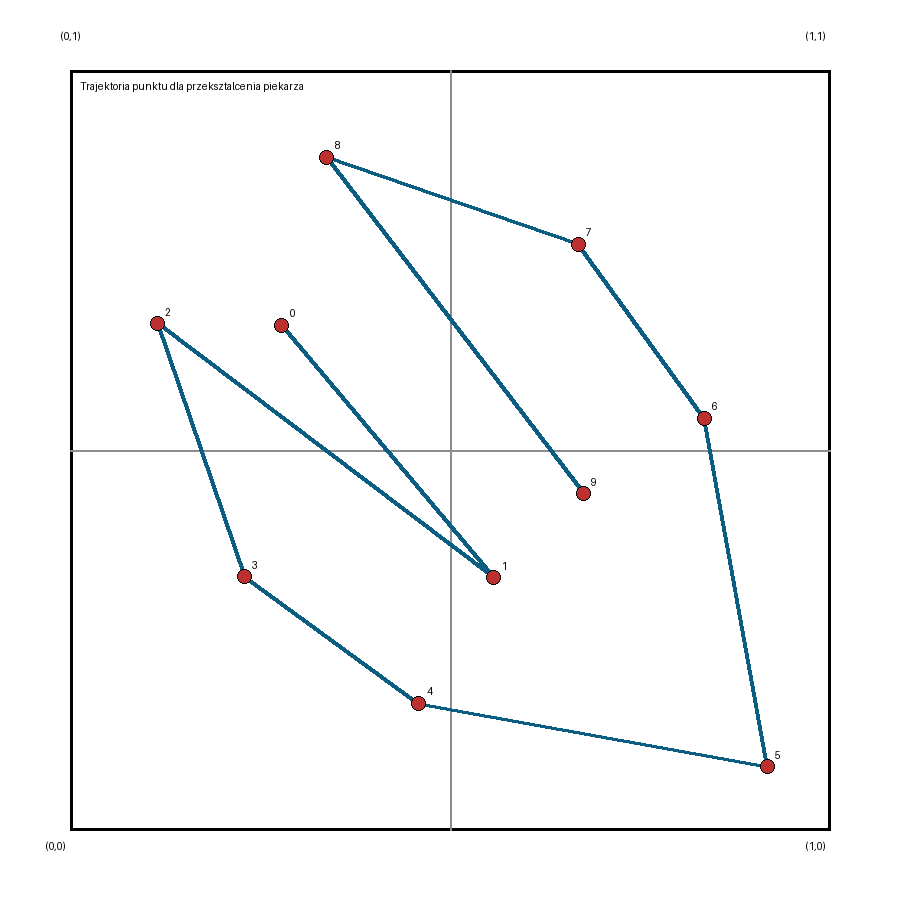
\includegraphics[width=0.72\textwidth]{figures/zadanie2_trajektoria.png}
\end{center}

\subsection*{4. Obraz przedstawiaj\k{a}cy Morskie Oko i jego iteracje}

Wewn\k{a}trz kwadratu \([0,1]^2\) umieszczamy prosty, stylizowany obraz przedstawiaj\k{a}cy Morskie Oko.
Nast\k{e}pnie wyznaczamy jego kolejne obrazy przez \(B, B^2, B^3, B^4\) oraz \(B^5\). Dzia\l anie
przekszta\l cenia jest bardzo dobrze widoczne: obraz zostaje wielokrotnie rozcinany, rozci\k{a}gany
i uk\l adany warstwowo.

\begin{center}
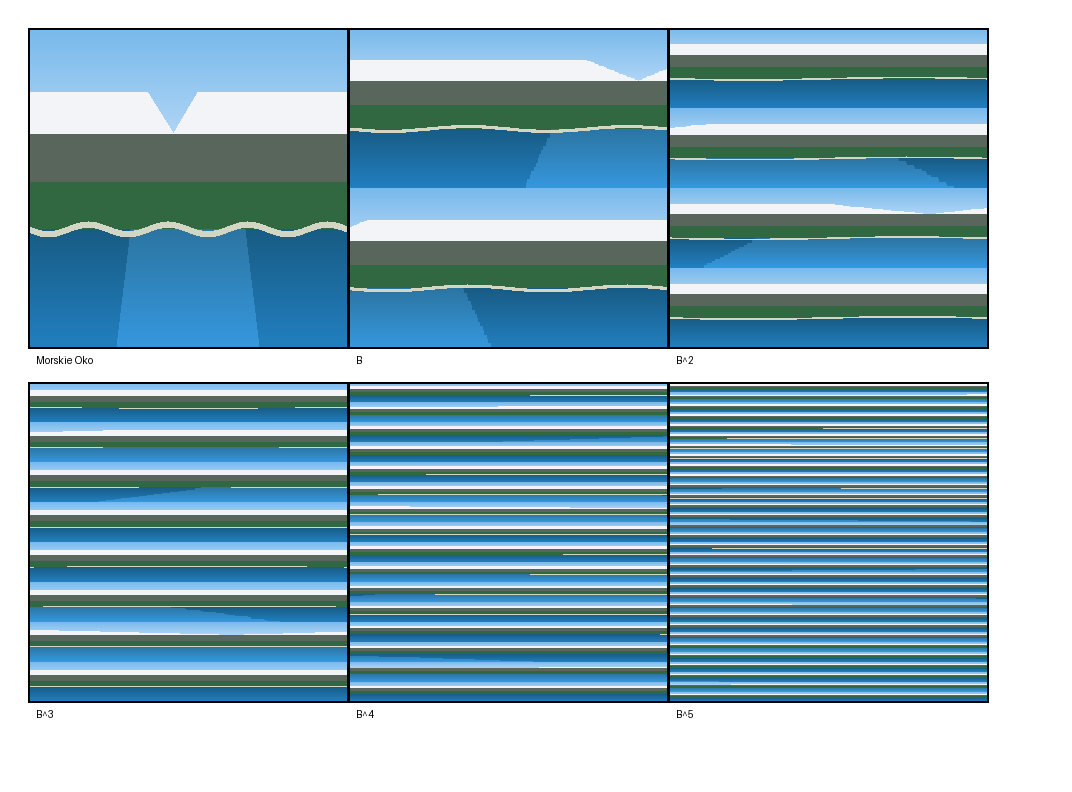
\includegraphics[width=0.95\textwidth]{figures/zadanie2_iteracje.png}
\end{center}

\subsection*{5. Skrypt w Pythonie}

Wszystkie obliczenia i rysunki zosta\l y wykonane skryptem
\texttt{scripts/zadanie2\_baker.py}. Program:
\begin{itemize}
    \item definiuje przekszta\l cenie piekarza,
    \item losuje punkt pocz\k{a}tkowy i wyznacza jego trajektori\k{e},
    \item tworzy prosty obraz inspirowany Morskim Okiem,
    \item generuje obrazy po iteracjach \(B, B^2, \dots, B^5\),
    \item zapisuje gotowe rysunki do plik\'ow graficznych.
\end{itemize}

Znaczenie najwa\.zniejszych fragment\'ow kodu jest nast\k{e}puj\k{a}ce:
\begin{itemize}
    \item funkcja \texttt{baker\_map} realizuje wz\'or na przekszta\l cenie piekarza,
    \item funkcja \texttt{iterate\_point} oblicza kolejne punkty trajektorii,
    \item funkcja \texttt{create\_morskie\_oko} buduje bazowy obraz wewn\k{a}trz kwadratu,
    \item funkcja \texttt{baker\_inverse\_image} oblicza kolejne iteracje obrazu.
\end{itemize}

Pe\l ny kod programu zamieszczono w aneksie na ko\'ncu dokumentu, aby by\l czytelny r\'ownie\.z w wersji PDF.

\subsection*{6. Dow\'od zachowania miary}

Poka\.zemy, \.ze przekszta\l cenie piekarza zachowuje pole, czyli dla dowolnego mierzalnego zbioru
\(A \subset [0,1)^2\) zachodzi
\[
    \Leb(B(A))=\Leb(A).
\]

Rozbijmy zbi\'or \(A\) na dwie cz\k{e}\'sci:
\[
    A_0 = A \cap \left([0,\tfrac{1}{2}) \times [0,1)\right), \qquad
    A_1 = A \cap \left([\tfrac{1}{2},1) \times [0,1)\right).
\]
Wtedy \(A=A_0 \cup A_1\), przy czym zbiory te s\k{a} roz\l \k{a}czne.

Na pierwszej po\l owie kwadratu odwzorowanie jest afiniczne:
\[
    B_0(x,y)=(2x,\tfrac{y}{2}),
\]
a jego macierz Jacobiego ma posta\'c
\[
    DB_0=
    \begin{pmatrix}
        2 & 0\\
        0 & \tfrac{1}{2}
    \end{pmatrix},
    \qquad
    \abs{\det DB_0}=1.
\]
Zatem \(\Leb(B(A_0))=\Leb(A_0)\).

Na drugiej po\l owie kwadratu mamy
\[
    B_1(x,y)=(2x-1,\tfrac{y+1}{2}),
\]
czyli znowu przekszta\l cenie afiniczne o tej samej macierzy liniowej:
\[
    DB_1=
    \begin{pmatrix}
        2 & 0\\
        0 & \tfrac{1}{2}
    \end{pmatrix},
    \qquad
    \abs{\det DB_1}=1.
\]
St\k{a}d otrzymujemy \(\Leb(B(A_1))=\Leb(A_1)\).

Ponadto obrazy tych dw\'och cz\k{e}\'sci s\k{a} roz\l \k{a}czne, poniewa\.z
\[
    B(A_0) \subset [0,1) \times [0,\tfrac{1}{2}),
    \qquad
    B(A_1) \subset [0,1) \times [\tfrac{1}{2},1).
\]
Mo\.zemy zatem doda\'c miary:
\[
    \Leb(B(A))
    = \Leb(B(A_0)) + \Leb(B(A_1))
    = \Leb(A_0) + \Leb(A_1)
    = \Leb(A).
\]
To ko\'nczy dow\'od.

\end{rozwiazaniebox}

\begin{wynikbox}
Przekszta\l cenie piekarza ma wz\'or
\[
    B(x,y)=
    \begin{cases}
    (2x,\tfrac{y}{2}), & x<\tfrac{1}{2},\\
    (2x-1,\tfrac{y+1}{2}), & x\ge \tfrac{1}{2},
    \end{cases}
\]
a dla punktu pocz\k{a}tkowego \((0.278662,\,0.664184)\) wyznaczyli\'smy trajektori\k{e}
\((x_n,y_n)=B^n(x_0,y_0)\) dla \(n=0,\dots,9\). Dodatkowo pokazali\'smy, jak przekszta\l cenie dzia\l a
na obraz, generuj\k{a}c kolejne iteracje stylizowanego rysunku Morskiego Oka, oraz udowodnili\'smy,
\.ze odwzorowanie zachowuje miar\k{e}, czyli pole.
\end{wynikbox}

\section{Zadanie 3}

\begin{opisbox}
Rozpatrujemy przekszta\l cenie pi\l okszta\l tne \(P\) oraz przekszta\l cenie namiotowe \(T\), wyznaczamy
ich punkty szczeg\'olne i opisujemy dzia\l anie iteracji w zapisie dw\'ojkowym.
\end{opisbox}

\begin{rozwiazaniebox}
\subsection*{1. Definicje przekszta\l ce\'n}

Przekszta\l cenie pi\l okszta\l tne \(P \colon [0,1] \to [0,1]\) jest dane wzorem
\[
P(x)=
\begin{cases}
2x, & \text{gdy } 0 \le x < \tfrac{1}{2},\\[0.3em]
2x-1, & \text{gdy } \tfrac{1}{2} \le x \le 1.
\end{cases}
\]

Przekszta\l cenie namiotowe \(T \colon [0,1] \to [0,1]\) ma posta\'c
\[
T(x)=1-\abs{1-2x}=
\begin{cases}
2x, & \text{gdy } 0 \le x < \tfrac{1}{2},\\[0.3em]
2-2x, & \text{gdy } \tfrac{1}{2} \le x \le 1.
\end{cases}
\]

\subsection*{2. Punkty sta\l e przekszta\l cenia \(T\)}

Szukamy rozwi\k{a}za\'n r\'ownania \(T(x)=x\).

Dla \(0 \le x < \tfrac{1}{2}\) mamy
\[
    2x=x \quad \Longrightarrow \quad x=0.
\]

Dla \(\tfrac{1}{2} \le x \le 1\) otrzymujemy
\[
    2-2x=x \quad \Longrightarrow \quad 2=3x \quad \Longrightarrow \quad x=\frac{2}{3}.
\]

Zatem zbi\'or punkt\'ow sta\l ych jest r\'owny
\[
    \Fix(T)=\set{0,\frac{2}{3}}.
\]

\subsection*{3. Stabilno\'s\'c punkt\'ow sta\l ych}

Na obu ga\l \k{e}ziach odwzorowania pochodna ma warto\'s\'c
\[
    T'(x)=
    \begin{cases}
        2, & x<\tfrac{1}{2},\\
        -2, & x>\tfrac{1}{2}.
    \end{cases}
\]
W obu przypadkach modu\l pochodnej jest r\'owny \(2\), a wi\k{e}c jest wi\k{e}kszy od \(1\).

W szczeg\'olno\'sci:
\[
    \abs{T'(0)}=2>1,
    \qquad
    \abs{T'\!\left(\frac{2}{3}\right)}=2>1.
\]

Oba punkty sta\l e s\k{a} zatem niestabilne, a dok\l adniej odpychaj\k{a}ce.

\subsection*{4. Wszystkie orbity d\l ugo\'sci \(2\)}

Szukamy punkt\'ow spe\l niaj\k{a}cych
\[
    T^2(x)=x,
\]
ale nieb\k{e}d\k{a}cych punktami sta\l ymi.

Najpierw wyznaczmy wz\'or na \(T^2\). Po rozbiciu przedzia\l u \([0,1]\) na cztery cz\k{e}\'sci dostajemy
\[
T^2(x)=
\begin{cases}
4x, & 0 \le x < \tfrac{1}{4},\\[0.3em]
2-4x, & \tfrac{1}{4} \le x < \tfrac{1}{2},\\[0.3em]
4x-2, & \tfrac{1}{2} \le x < \tfrac{3}{4},\\[0.3em]
4-4x, & \tfrac{3}{4} \le x \le 1.
\end{cases}
\]

Rozwi\k{a}zujemy kolejno r\'ownania:
\[
\begin{aligned}
4x=x &\Longrightarrow x=0,\\
2-4x=x &\Longrightarrow x=\frac{2}{5},\\
4x-2=x &\Longrightarrow x=\frac{2}{3},\\
4-4x=x &\Longrightarrow x=\frac{4}{5}.
\end{aligned}
\]

Po odrzuceniu punkt\'ow sta\l ych \(0\) oraz \(\tfrac{2}{3}\) zostaj\k{a} dwa punkty okresu zasadniczego \(2\):
\[
    \frac{2}{5}
    \qquad \text{oraz} \qquad
    \frac{4}{5}.
\]

Tworz\k{a} one jedn\k{a} orbit\k{e} d\l ugo\'sci \(2\), poniewa\.z
\[
    T\!\left(\frac{2}{5}\right)=\frac{4}{5},
    \qquad
    T\!\left(\frac{4}{5}\right)=\frac{2}{5}.
\]

\subsection*{5. Stabilno\'s\'c orbity d\l ugo\'sci \(2\)}

Stabilno\'s\'c orbity dwucyklowej badamy za pomoc\k{a} pochodnej drugiej iteracji:
\[
    (T^2)'(x)=T'(T(x))\cdot T'(x).
\]

Dla punktu \(x=\tfrac{2}{5}\) mamy \(T'(x)=2\), natomiast
\[
    T\!\left(\frac{2}{5}\right)=\frac{4}{5},
    \qquad
    T'\!\left(\frac{4}{5}\right)=-2.
\]
Zatem
\[
    (T^2)'\!\left(\frac{2}{5}\right)=(-2)\cdot 2=-4.
\]
Wobec tego
\[
    \abs{(T^2)'\!\left(\frac{2}{5}\right)}=4>1.
\]

Tak samo dla drugiego punktu orbity:
\[
    \abs{(T^2)'\!\left(\frac{4}{5}\right)}=4>1.
\]
Oznacza to, \.ze orbita d\l ugo\'sci \(2\) jest niestabilna.

\subsection*{6. Wykres paj\k{e}czynowy}

Do zilustrowania cyklu \(\set{\tfrac{2}{5},\tfrac{4}{5}}\) przygotowano wykres paj\k{e}czynowy.
Na wykresie zaznaczono prost\k{a} \(y=x\), wykres funkcji \(y=T(x)\) oraz dwie trajektorie
startuj\k{a}ce z punkt\'ow \(\tfrac{2}{5}\) i \(\tfrac{4}{5}\).

\begin{center}
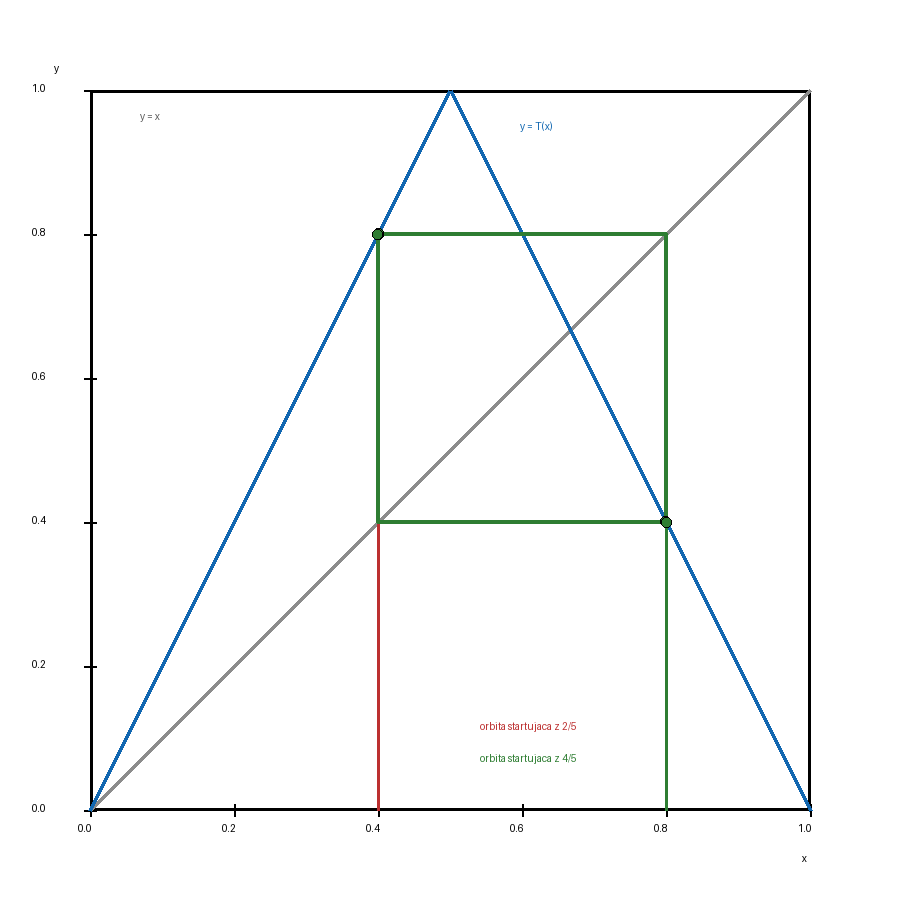
\includegraphics[width=0.72\textwidth]{figures/zadanie3_pajeczyna.png}
\end{center}

\subsection*{7. Skrypt w Pythonie}

Rysunek zosta\l wygenerowany skryptem \texttt{scripts/zadanie3\_tent.py}. Program:
\begin{itemize}
    \item definiuje odwzorowanie namiotowe,
    \item tworzy wykres funkcji \(T\) oraz prostej \(y=x\),
    \item rysuje paj\k{e}czyn\k{e} dla orbity startuj\k{a}cej z \(\tfrac{2}{5}\) i \(\tfrac{4}{5}\),
    \item zapisuje gotowy rysunek do pliku graficznego.
\end{itemize}

Pe\l ny kod programu zamieszczono w aneksie na ko\'ncu dokumentu, aby by\l czytelny r\'ownie\.z w wersji PDF.

\subsection*{8. Dzia\l anie przekszta\l cenia \(P\) w zapisie dw\'ojkowym}

Niech
\[
    x=(0,a_1a_2a_3\ldots)_2,
\]
przy czym pomijamy liczby o dw\'och rozwini\k{e}ciach dw\'ojkowych.

Je\.zeli \(a_1=0\), to \(x<\tfrac{1}{2}\), a zatem
\[
    P(x)=2x=(0,a_2a_3a_4\ldots)_2.
\]

Je\.zeli \(a_1=1\), to \(x\ge \tfrac{1}{2}\), wi\k{e}c
\[
    P(x)=2x-1=(0,a_2a_3a_4\ldots)_2.
\]

W obu przypadkach przekszta\l cenie \(P\) usuwa pierwszy bit rozwini\k{e}cia dw\'ojkowego. Otrzymujemy
wi\k{e}c przesuni\k{e}cie Bernouliego:
\[
    \sigma((0,a_1a_2a_3\ldots)_2)=(0,a_2a_3a_4\ldots)_2.
\]

\subsection*{9. Dow\'od wzoru \(T^n = T \circ P^{n-1}\)}

Najpierw poka\.zemy, \.ze
\[
    T^2=T\circ P.
\]

Sprawdzamy to na czterech przedzia\l ach:
\[
\begin{array}{c|c|c}
\text{przedzia\l} & T(T(x)) & T(P(x)) \\ \hline
\bigl[0,\tfrac{1}{4}\bigr) & 4x & 4x \\
\bigl[\tfrac{1}{4},\tfrac{1}{2}\bigr) & 2-4x & 2-4x \\
\bigl[\tfrac{1}{2},\tfrac{3}{4}\bigr) & 4x-2 & 4x-2 \\
\bigl[\tfrac{3}{4},1\bigr] & 4-4x & 4-4x
\end{array}
\]
Zatem rzeczywi\'scie \(T^2=T\circ P\).

Teraz przeprowadzamy indukcj\k{e} po \(n\).

Dla \(n=1\) mamy
\[
    T^1=T=T\circ P^0.
\]

Za\l \'o\.zmy, \.ze dla pewnego \(n\ge 1\) zachodzi
\[
    T^n=T\circ P^{n-1}.
\]
Wtedy
\[
    T^{n+1}
    = T^2 \circ P^{n-1}
    = (T\circ P)\circ P^{n-1}
    = T\circ P^n.
\]
To ko\'nczy dow\'od indukcyjny.

\subsection*{10. Opis dzia\l ania iteracji \(T^n\) na rozwini\k{e}ciach dw\'ojkowych}

Z punktu 8 wiemy, \.ze
\[
    P^{n-1}(x)=(0,a_na_{n+1}a_{n+2}\ldots)_2.
\]
Korzystaj\k{a}c z punktu 9, dostajemy
\[
    T^n(x)=T(P^{n-1}(x)).
\]

Je\.zeli \(a_n=0\), to \(P^{n-1}(x)<\tfrac{1}{2}\), a wi\k{e}c
\[
    T^n(x)=2P^{n-1}(x)=(0,a_{n+1}a_{n+2}a_{n+3}\ldots)_2.
\]

Je\.zeli natomiast \(a_n=1\), to \(P^{n-1}(x)\ge \tfrac{1}{2}\), zatem
\[
    T^n(x)=2-2P^{n-1}(x)
    =1-(0,a_{n+1}a_{n+2}a_{n+3}\ldots)_2.
\]

Ostatecznie iteracja \(T^n\) dzia\l a na rozwini\k{e}ciu dw\'ojkowym w spos\'ob nast\k{e}puj\k{a}cy:
\[
T^n\bigl((0,a_1a_2a_3\ldots)_2\bigr)=
\begin{cases}
(0,a_{n+1}a_{n+2}a_{n+3}\ldots)_2, & \text{gdy } a_n=0,\\[0.4em]
1-(0,a_{n+1}a_{n+2}a_{n+3}\ldots)_2, & \text{gdy } a_n=1.
\end{cases}
\]

Interpretacja jest bardzo prosta: po \(n-1\) przesuni\k{e}ciach przez \(P\) patrzymy na \(n\)-ty bit.
Je\.zeli jest on r\'owny \(0\), otrzymujemy zwyk\l e przesuni\k{e}cie; je\.zeli jest r\'owny \(1\),
to po przesuni\k{e}ciu nast\k{e}puje odbicie wzgl\k{e}dem punktu \(\tfrac{1}{2}\).

\end{rozwiazaniebox}

\begin{wynikbox}
Dla przekszta\l cenia namiotowego \(T\) punktami sta\l ymi s\k{a} \(0\) oraz \(\tfrac{2}{3}\), przy czym
oba s\k{a} niestabilne. Jedyna orbita d\l ugo\'sci \(2\) ma posta\'c
\[
    \frac{2}{5} \longleftrightarrow \frac{4}{5},
\]
i r\'ownie\.z jest odpychaj\k{a}ca. Z kolei przekszta\l cenie pi\l okszta\l tne \(P\) usuwa pierwszy bit
rozwini\k{e}cia dw\'ojkowego, czyli realizuje przesuni\k{e}cie Bernouliego, a iteracje namiotowe spe\l niaj\k{a}
wz\'or \(T^n=T\circ P^{n-1}\).
\end{wynikbox}

\clearpage
\section{Aneks: Kody Python}

W tym aneksie zebrano wszystkie skrypty wykorzystane do generowania wynik\'ow, rysunk\'ow
i przyk\l ad\'ow pojawiaj\k{a}cych si\k{e} w zadaniach. Umieszczamy je poza kolorowymi ramkami,
aby by\l y w pe\l ni widoczne w pliku PDF.

\subsection{Kod do zadania 1}

Skrypt \texttt{scripts/zadanie1\_markov.py} analizuje melodi\k{e}, buduje macierz liczebno\'sci
przej\'s\'c, wyznacza macierz przej\'scia \l a\'ncucha Markowa, a nast\k{e}pnie generuje now\k{a}
melodi\k{e} tej samej d\l ugo\'sci.

\lstinputlisting[
    language=Python,
    caption={Kod do zadania 1: \l a\'ncuch Markowa dla melodii}
]{scripts/zadanie1_markov.py}

\subsection{Kod do zadania 2}

Skrypt \texttt{scripts/zadanie2\_baker.py} definiuje przekszta\l cenie piekarza, losuje punkt
pocz\k{a}tkowy, wyznacza jego trajektori\k{e} oraz generuje obrazy przedstawiaj\k{a}ce kolejne iteracje
stylizowanego rysunku Morskiego Oka.

\lstinputlisting[
    language=Python,
    caption={Kod do zadania 2: przekszta\l cenie piekarza}
]{scripts/zadanie2_baker.py}

\subsection{Kod do zadania 3}

Skrypt \texttt{scripts/zadanie3\_tent.py} rysuje wykres przekszta\l cenia namiotowego, prost\k{a}
\(y=x\) oraz wykresy paj\k{e}czynowe dla orbity dwucyklowej \(\{\tfrac{2}{5},\tfrac{4}{5}\}\).

\lstinputlisting[
    language=Python,
    caption={Kod do zadania 3: wykres paj\k{e}czynowy dla odwzorowania namiotowego}
]{scripts/zadanie3_tent.py}

\end{document}
